\section{Thảo luận và kết luận}

\begin{frame}{Hai chế độ dữ liệu - Bài học chung}
\centering
\vspace{0.15cm}
\begin{tikzpicture}[
 stage/.style={draw=PrimaryBlue,rounded corners=5pt,fill=PaleBlue,
 minimum height=1.78cm,text width=3.0cm,align=center,font=\small,inner sep=7pt},
 arr/.style={-Latex,draw=PrimaryBlue,line width=1.4pt}]
\node[stage] (a) {\bfseries Dữ liệu đủ dày\\[2pt]$d=1$\\[4pt]Tốt nhất mỗi nhóm vượt MostPop \textbf{54--60\%}};
\node[stage,right=0.44cm of a] (b) {\bfseries Dữ liệu giảm\\[2pt]$d=0{,}5$\\[4pt]Chỉ \textbf{DFHF} còn vượt MostPop (11\%)};
\node[stage,right=0.44cm of b] (c) {\bfseries Rất thưa\\[2pt]$d=0{,}25$\\[4pt]\textbf{Không mô hình nào} hơn MostPop};
\draw[arr] (a) -- (b);\draw[arr] (b) -- (c);
\end{tikzpicture}
\vspace{0.39cm}

\begin{columns}[T,onlytextwidth]

    \begin{column}{0.47\textwidth}
        \begin{block}{GRNR: Thiếu kết nối}
            \small
            Chỉ còn \textbf{4,2\%} cặp đồng xuất hiện. Ít láng giềng để học hệ số.
        \end{block}
    \end{column}

    \hfill

    \begin{column}{0.47\textwidth}
        \begin{block}{DFHF: Lùi về chặn}
            \small \textbf{68\%} người dùng chỉ còn 1 tương tác: xếp hạng bằng $b_i$.
        \end{block}
    \end{column}

\end{columns}
\vspace{0.18cm}
\takeaway{Trên dữ liệu này, \textbf{độ dày dữ liệu} quyết định lợi ích cá nhân hóa nhiều hơn việc chọn một mô hình phức tạp.}
\end{frame}

\begin{frame}{Demo: Gợi ý cho người dùng có sẵn}
\centering

\vspace{-0.06cm}

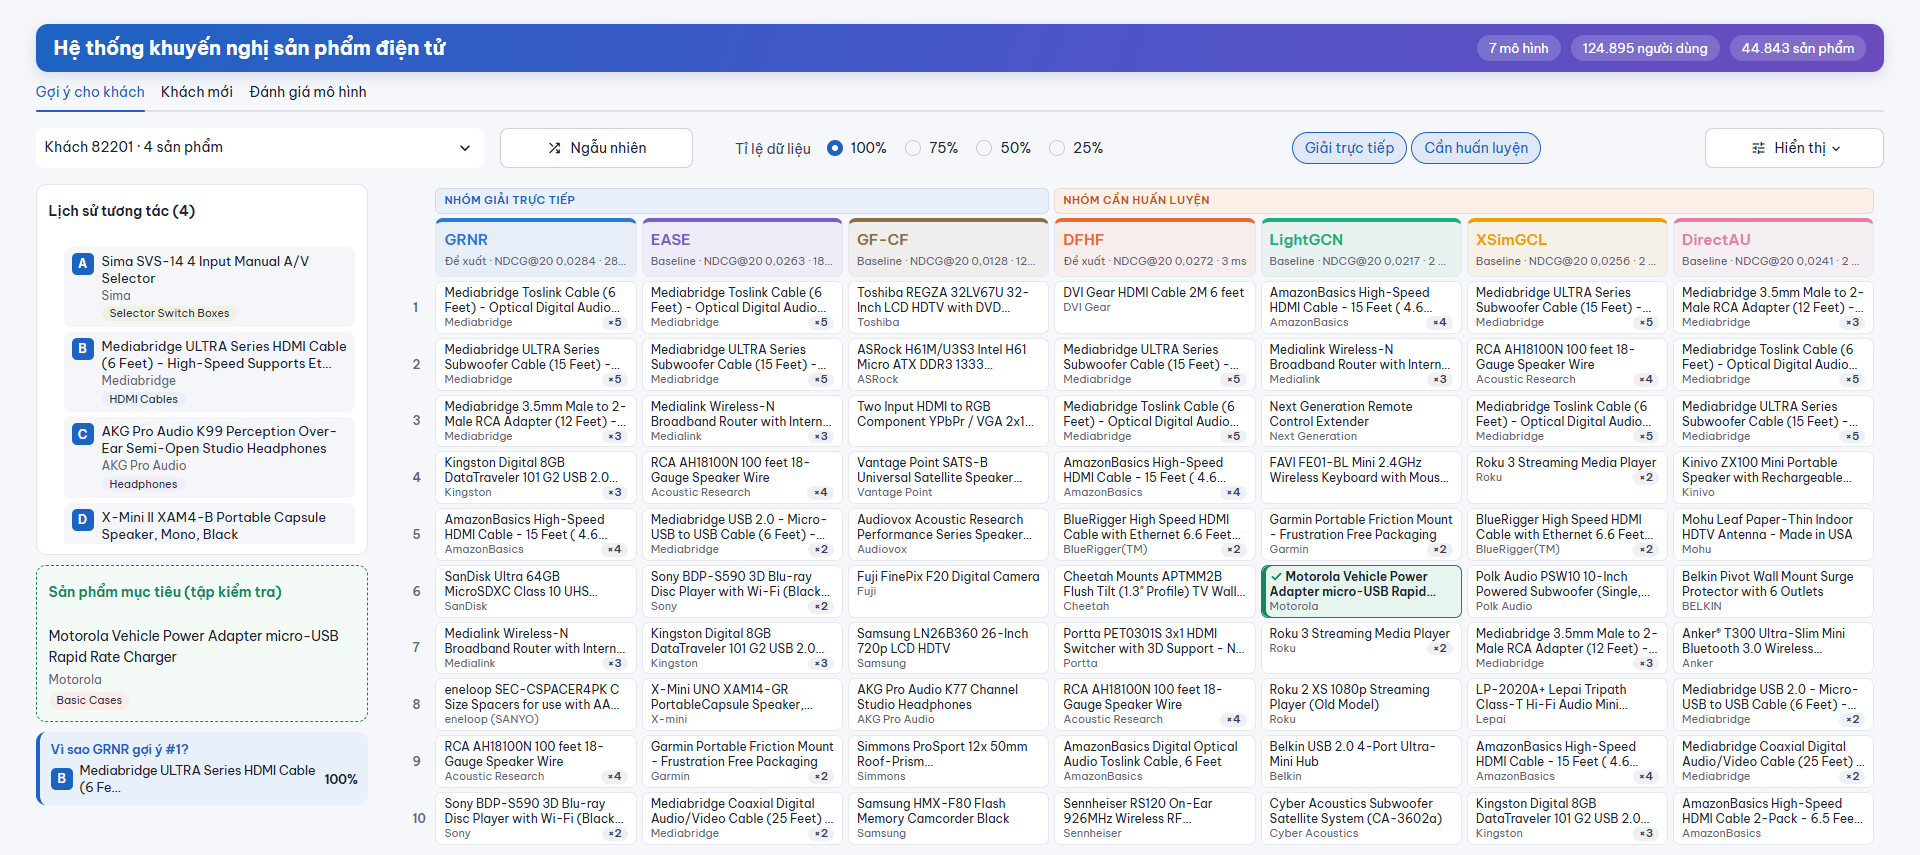
\includegraphics[
    width=\linewidth,
    height=0.66\textheight,
    keepaspectratio
]{figures/anh_1.png}

\vspace{0.05cm}

\takeaway{
Từ lịch sử của người dùng, hệ thống hiển thị
\textbf{Top-10 của 7 mô hình} và sản phẩm mục tiêu.
Với GRNR, ô ``Vì sao gợi ý \#1?''
thể hiện đóng góp từ các sản phẩm trong lịch sử.
}

\end{frame}

\begin{frame}{Demo: Gợi ý cho khách mới}
\centering

\vspace{-0.06cm}

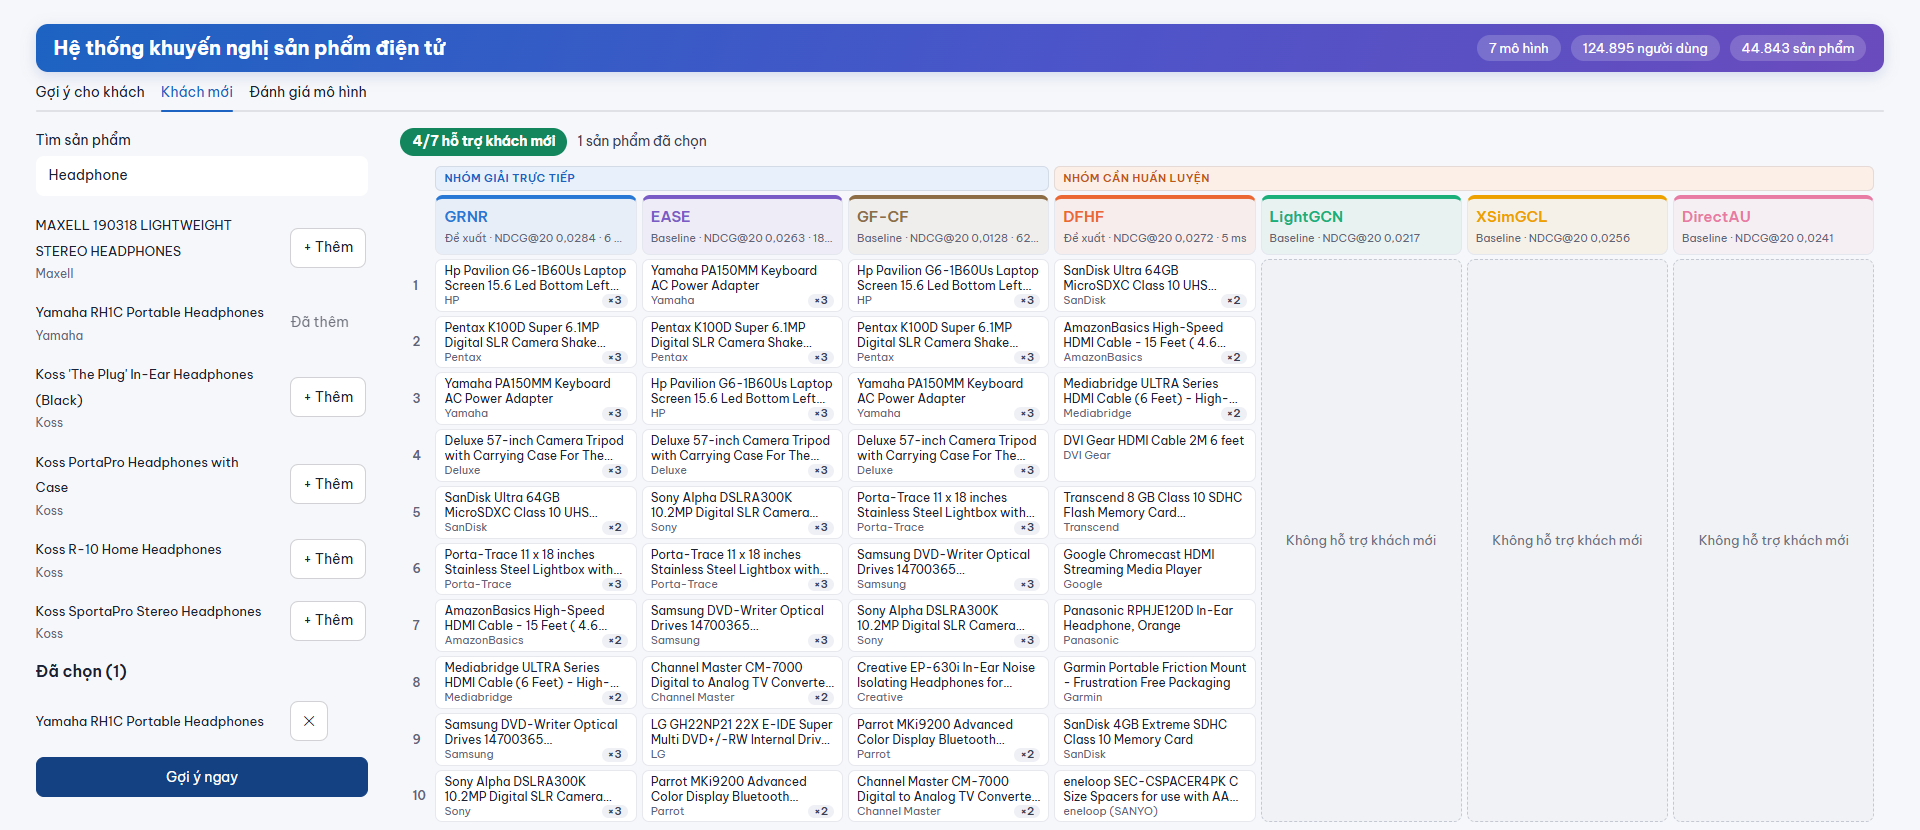
\includegraphics[
    width=\linewidth,
    height=0.66\textheight,
    keepaspectratio
]{figures/anh_2.png}

\vspace{0.05cm}

\takeaway{
Khách mới có thể \textbf{tìm và thêm sản phẩm}
để tạo lịch sử.
\textbf{4/7 mô hình} chấm điểm lịch sử mới
mà không huấn luyện lại;
trong ví dụ một tương tác,
DFHF xếp hạng theo hệ số chặn $b_i$.
}

\end{frame}

\begin{frame}{Demo: Gợi ý và lý do gợi ý của GRNR}
\centering
\begin{columns}[T,totalwidth=\textwidth]
\column{0.50\textwidth}
\centering
{\footnotesize\bfseries\color{PrimaryBlue}Sản phẩm mục tiêu và lý do GRNR gợi ý}\par\vspace{0.13cm}
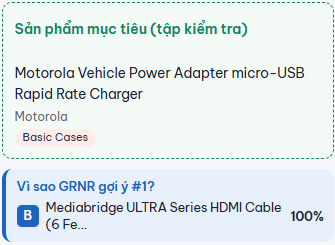
\includegraphics[width=0.96\linewidth,height=0.53\textheight,keepaspectratio]{figures/demo_focus_reason.png}

\column{0.48\textwidth}
\centering
{\footnotesize\bfseries\color{PrimaryBlue}Top-3 gợi ý của GRNR}\par\vspace{0.13cm}
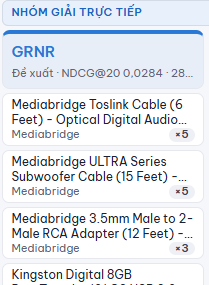
\includegraphics[width=0.98\linewidth,height=0.53\textheight,keepaspectratio]{figures/demo_focus_grnr_top3.png}
\end{columns}
\vspace{0.09cm}
\takeaway{Từ lịch sử 4 tương tác, demo dùng checkpoint sẵn có để xếp hạng. Ô ``Vì sao GRNR gợi ý \#1?'' cho thấy đóng góp từ lịch sử, \textbf{không} là diễn giải nhân quả.}
\end{frame}

\begin{frame}{Kết luận gắn với bốn câu hỏi nghiên cứu}
\small
\begin{enumerate}\setlength\itemsep{0.29cm}
\item \textbf{Chất lượng:} GRNR hơn EASE top-128; chưa chứng minh hơn EASE đầy đủ. DFHF dẫn đầu nhóm cần huấn luyện trên test.
\item \textbf{Dữ liệu thưa:} ở $d=0{,}25$, \textbf{không mô hình nào hơn MostPop}; lợi thế DFHF chủ yếu từ hệ số chặn.
\item \textbf{Chi phí:} GRNR nhỏ hơn EASE đầy đủ \textbf{khoảng 190 lần}; DFHF huấn luyện chậm nhất nhóm, nhạy checkpoint.
\item \textbf{Lịch sử mới:} cả hai phương pháp tính được điểm không cần huấn luyện lại; demo minh họa phân rã điểm GRNR.
\end{enumerate}
\vspace{0.12cm}
\takeaway{Kết quả đo trên \textbf{test độc lập}, nhưng chỉ với một bộ dữ liệu và một seed, nên vẫn là \textbf{kết quả khám phá}.}
\end{frame}

\begin{frame}{Hạn chế quan trọng và ưu tiên tiếp theo}
\small

\begin{columns}[T,onlytextwidth]

    \begin{column}{0.49\textwidth}
        \begin{block}{Cần thận trọng}
            \begin{itemize}\setlength\itemsep{6pt}
            \item \textbf{Một bộ dữ liệu, một seed}
            \item Ngân sách \textbf{tinh chỉnh baseline không cân bằng}
            \item \textbf{DirectAU có dấu hiệu chưa hội tụ}
            \item \textbf{GF-CF thấp bất thường}: cần kiểm tra cài đặt/cấu hình
            \end{itemize}
        \end{block}
    \end{column}

    \hfill

    \begin{column}{0.47\textwidth}
        \begin{block}{Ưu tiên phát triển}
            \begin{enumerate}\setlength\itemsep{6pt}
            \item Nhiều seed, thêm bộ dữ liệu.
            \item Kiểm lại GF-CF; tuning cùng ngân sách, huấn luyện DirectAU đủ lâu.
            \item Ablation từng thành phần GRNR/DFHF.
            \item Kết hợp \textbf{MostPop dự phòng} khi lịch sử quá ngắn.
            
            \end{enumerate}
        \end{block}
    \end{column}

\end{columns}


\vspace{0.18cm}
\vspace{0.18cm}
\begin{center}
\begin{minipage}{0.91\textwidth}
\centering\footnotesize\bfseries\color{PrimaryBlue}
Cần kiểm chứng: phương án dự phòng và khả năng khái quát sang dữ liệu khác.
\end{minipage}
\end{center}
\end{frame}

\begin{frame}[plain]
\vfill
\begin{center}
{\LARGE\bfseries\color{PrimaryBlue}XIN CẢM ƠN THẦY CÔ VÀ CÁC BẠN!}\\[0.65cm]
{\large Nhóm sẵn sàng trao đổi và trả lời câu hỏi.}\\[0.32cm]
{\normalsize Hệ thống khuyến nghị sản phẩm điện tử\\
bằng hồi quy lân cận và khuếch tán trên đồ thị}
\end{center}
\vfill
\end{frame}
